\chapter{Techniques utilisées}

   \section{R-CNN}

    \subsection{Principes}
      
      En vue d'aborder les problèmes de détection et de localisation d'objets, nous avons misé sur deux techniques disctintes d'analyse d'images au travers de réseaux neuronaux : 
      \begin{itemize}
       \item La proposition de régions d'intérêt (Region Proposal Network, ou RPN)
       \item La classification d'objets au sein de ces régions (CNN)
      \end{itemize}
      
      Ces deux techniques se retrouvent au sein de l'algorithme R-CNN\cite{Bib_RCNN} (Region-based CNN) implémenté en Matlab.
      Comme son nom l'indique, R-CNN tire parti de la localisation de regions d'intérêt (Region of Interest ou ROI) avant de procéder à la classification. 
      Le réseau dédié à la classification opère de manière quasi-analogue à ce que nous avons décrit précédemment pour ses premières couches. Avant les couches entièrement connectées (qui calculent
      la sortie du réseau) est intercalé le RPN. 
      Ce dernier va interpréter les résultats des convolutions en vue de soumettre un selection de régions où les objets d'intérêt sont susceptibles de se trouver. 
      Celui-ci est capable dans le même temps d'estimer la présence ou non d'un objet (objectness score) et d'en donner les limites en tout point de l'image. 
      La sortie du RPN est constituée de ces régions qui seront ensuite traîtées par les couches pleinement connectées afin de donner les résultats de la classification. 
      L'ensemble de la chaîne fait appel à plusieurs couches de convolution et est entraînable. 
      La figure suivante établit le récapitulatif de ce fonctionnement.  
      
      \begin{figure}[H]
	  \centering
	  \makebox[\textwidth]{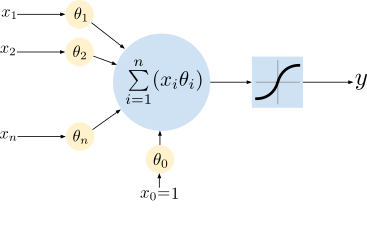
\includegraphics[width=.5\paperwidth]{c2p1s1_rcnn}}
	  \caption{ Principe d'un \gls{R-CNN} }
	  \label{fig:c2p1s1_rcnn}
      \end{figure}
     
      
    \subsection{Approche pratique}
    
      En pratique, R-CNN a ouvert le champs à des recherches connexes visant notamment à en reprendre les principes fondateurs tout en améliorant sa vitesse de traitement \cite{Bib_FastRCNN}. 
      Nous avons retenu pour ce travail Faster-RCNN\cite{Bib_FasterRCNN}, qui est à notre connaissance l'implémentation la plus récente basée sur R-CNN. 
      Nativement implémentée en Python et en Matlab ce travail s'oriente, comme ses prédecesseurs, vers l'application de CNN à la classification et à la détection d'objets.  
      
      La classification est assurée grâce à la bibliothèque open-source Caffe, développée
      par Berkley Vision and Learning Center (BVLC)\cite{Bib_CaffeHome}. Une documentation complète du framework est disponible sur le site internet 
      officiel\cite{Bib_CaffeTuto}, décrivant notamment les éléments de référence afin de concevoir, entraîner et tester des réseaux de neurones. 
      
      L'avancée majeure de Faster R-CNN concerne la chaîne de détection, qui peut se dérouler en quasi temps-réel. 
      En effet, les précédentes incarnations de l'algorithme étaient freinées par le temps nécessaire en amont de la détection, à savoir la proposition de régions d'intérêt. 
      Parmi les méthodes de propositions de régions les plus connues, on trouve celles tirées de conversion de l'image en superpixels, ou encore celles basées sur le glissement d'une fenêtre sur la surface à traiter. 
      L'approche adoptée par Fast et Faster R-CNN est différente. 
      Elle vise à séparer le problème de proposition d'objet de celui de détection de l'objet, tout en mutualisant un certain nombre de données entre ces deux facettes. 
      Le framework employé va donc être composé de plusieurs modules aux objectifs disctincts (qui peuvent être mis en prallèle avec ceux décrits précédemment) : 
      
      \begin{itemize}
       \item Un module RPN (Region Proposal Network)
       \item Un module de classification d'objet basé sur la bibliothèque Caffe
      \end{itemize}
      
      Dans Faster R-CNN, les cartes de caractéritiques résultant de la convolution sont mises au service de suggestions de régions délimitant un objet (region proposal) au sein de l'image. Le réseau se voit également
      complété d'un RPN (Region Proposal Network). Un RPN est un type de CNN capable simultanément d'estimer la présence ou non d'un objet (objectness score) et d'en donner les limites, en tout point de l'image.
      Un RPN est entraînable de bout-en-bout. 
      
      L'objectif d'optimisation liée à la detection d'objets est atteint par le framework, 
      puisqu'on observe une réduction du goulet d'étranglement représenté par la proposition de régions d'intérêt à 0.01 seconde par image sur GPU (sur PASCAL VOC). 
      Une autre évolution introduite par Faster R-CNN et RPN consiste à alterner l'utilisation des deux premiers modules, tout en partageant les caractéritiques résultant des convolutions respectives. 
      
      Notons également que depuis sa publication en 2015, Faster R-CNN et RPN ont compté sur plusieurs premières places à des compétitions internationales, des applications dans divers domaines tels que la détection
      d'objets 3D ou encore l'intégration à des produits commerciaux grands publics tels que Pinterest. 
      
      Dans le cadre de ce travail, nous avons eu à réaliser une interface qui nous permette d'utiliser les fonctionnalités de Faster R-CNN en C++. 
      Elle vise à manipuler les données entrantes et sortantes de le framework Caffe, afin d'exploiter les réseaux de neurones adaptés au modèle de Faster R-CNN,   
      Pour ce faire, nous nous sommes basés sur son impélmentation originale en Python, ainsi que sur divers travaux issus du web \cite{Bib_FasterRCNN_encapsulation}.  
      
      \section{Suivi d'objets}

	\subsection{Histogramme de gradient}
	\subsection{Background Foreground}
    
      \section{SURF}

	\subsection{Principes}
	
	SURF, pour Speeded-Up Robust Features, est une technique de reconnaissance d'objets tirés de scènes différentes inventée par Bay Herbert, Tuytelaars Tinne et Van Gool Luc \cite{Bib_SURF}.
	L'action de SURF s'effectue en deux temps -la détection de points d'intérêts d'une scène et le calcul de leurs descripteurs-  que nous allons brièvement évoquer ici. 
	
	Le premier point s'appuie sur un calcul d'\gls{intimg} qui permettra de réduire les temps de calcul, et ceci de manière scalable au regard de la taille de l'image ou des filtres utilisés.
	Ici, l'image intégrale va entrer en jeu lors de la recherche de points d'intérêts à différentes échelles, les filtres de convolution utilisés étant de type ``box-filter''. 
	Au lieu de sous-échantillonner l'image d'entrée, on pourra jouer sur la taille des filtres qui seront appliqués à l'image d'origine et diminuer significativement le temps dédié à la recherche.  
	C'est une \gls{hessMat} (ou matrice Hessienne) qui permet de localiser des structures de type ``blob'' à une échelle donnée.
	Lorsque de tels déterminants sont calculés pour toutes les échelles de filtres fixées, les points d'intérêt détectés correspondent alors aux valeurs maximales ayant été trouvées. 
	
	Le deuxième point vise à extraire une description suffisamment robuste des points d'intérêt, permettant ensuite des comparaisons qui amènent le système à reconnaître un objet dans un scène à partir d'une image d'origine.
	La technique employée par SURF à cet égard consiste en trois étapes : 
	l'affectation d'une orientation aux points d'intérêt, la construction des descripteurs basés sur les réponses à des ondelettes de Haar et enfin, la comparaison basée sur un système d'indexation rapide.  
	
	L'orientation des points d'intérêt s'effectue en calculant pour chacun d'eux la réponse à des ondelettes de Haar distribuées selon les directions $x$ et $y$. Grâce à l'image intégrale, les réponses aux ondelettes ne requièrent que six opérations. 
	La réponse directionnelle trouvée est représentée au sein d'un cercle dont le rayon est proportionnel à l'échelle à laquelle le point à été trouvé. 
	L'extraction des descripteurs consiste à sommer les réponses aux ondelettes précédemment calculées. On somme notamment les réponses liées à la direction $x$ avec celles calculées en $y$, puis on effectue une moyenne sur une région donnée afin de
	minimiser le nombre de vecteurs résultants. Le vecteur de caractéristiques est donnée par : 
	\begin{center}
	    $ \overrightarrow{\mathcal{V}} = \left( \begin{array}{c}
	    \sum{dx}	\\
	    \sum{dy}	\\
	    \sum{|dx|}	\\
	    \sum{|dy|}	\\
	  \end{array} \right)$
	\end{center}

	La technique d'indexation employée reprend l'approximation de la matrice de Hesse précédemment calculée. Cette fois ci, c'est la trace de la matrice qui est utilisée, à savoir le Laplacien. Ce dernier donne des indications en termes de 
	luminosité de l'avant et de l'arrière plan, de telle sorte que la comparaison de deux points d'intérêt disposant de caractéristiques non similaires donne un résultat négatif. Autrement dit, un point d'intérêt sombre ne correspondra
	pas avec un point d'intérêt lumineux. Notons que cette étape ne demande pas de calculs supplémentaires puisqu'elle reprend les résultats obtenus lors de la recherche des points d'intérêt. Plus précisemment, 
	la signe positif ou négatif du Laplacien nous indique si nous sommmes dans une situation où l'avant plan est sombre et l'arrière plan brillant, ou si nous sommes dans la situation inverse. 
	
	Pour conclure, l'utilisation de SURF au sein de ce projet a été motivée par deux atouts majeurs : le premier étant la rapidité intrinsèque à l'algorithme avec notamment la possibilité de l'utiliser dans un contexte de temps réél, 
	le deuxième est sa robustesse aux changements d'échelle qui nous paraît appréciable lors de traitements de séquences filmées.
	
	\subsection{Approche pratique}
	
	Une implémentation de SURF est inclue dans la librairie OpenCV \cite{Bib_SURFOpenCV}. Depuis la version 3.0 de OpenCV, il est nécessaire d'importer la classe SURF depuis le dépôt opencv-contrib et particulièrement, depuis
	le module xfeatures2d. Cette partie évoque la façon dont nous l'avons employée et à quelles fins, sachant que l'utilisation de SURF a sensiblement changée dans la version 3.0 d'OpenCV.   
	
	Pour notre part, nous utiliserons SURF afin de calculer un score qui nous permettra d'apprécier le résultat du trackeur. Premièrement, nous fournissons à SURF la fenêtre contenant l'objet de référence que nous voulons suivre.
	A chaque nouvelle position détectée, nous demandons à SURF d'effectuer une détection des points d'intérêt correspondant à l'objet de référence, et ce sur la totalité de la nouvelle scène. Enfin, le score est donné par : 
	\begin{center} 
	  $ score = \dfrac{\text{Points d'intérêt dans la zone détectée}}{\text{Total des points d'intérêt}}$
	\end{center}
	
	Si le score n'atteint pas un certain seuil, nous lançons alors un re-détection qui fait cette fois appel au réseau de neurones (Faster R-CNN). Ce choix s'explique par la vitesse moindre du 
	réseau de neurones par rapport à celle du trackeur et, parallèlement, la qualité de détection supérieure de ce premier. Il nous fallait alors imaginer une technique qui permette d'utiliser Faster R-CNN dans un contexte pertinent, 
	à savoir lorsque la détection nous apparaît défaillante au travers de localisations de points d'intérêts fournis par SURF. 
	
	Le psoeudo-code suivant résume ce fonctionnement :
	
	\begin{lstlisting}
	
	// detection de l'objet d'interet grace au reseau de neurones
	object <- CNN_detection()
	// initialisation de SURF avec l'objet de reference
	surf.initialize( object )  
	
	Pour toute img dans flux_images faire : 
	  // on recupere la nouvelle position de l'objet 
	  objpos <- track( img )
	  // calcul du score d'apres le traitement de SURF
	  score <- surf.match( img, objpos )
	  
	  Si score < SCORE_THRESHOLD
	    // on lance une redetection avec le reseau de neurones
	    object <- CNN_detection()
	    // on reinitialise SURF
	    surf.initialize( object )
	  Fin si
	
	Fin pour
	
	\end{lstlisting}
	